\documentclass[11pt,conference]{IEEEtran}

\ifCLASSINFOpdf
\else
\fi

\usepackage{url}

% correct bad hyphenation here
\hyphenation{key-strokes}

\usepackage{graphicx}
\usepackage{multirow}

%\usepackage{titlesec}
%\titlespacing*{\section}{0pt}{.4\baselineskip}{.2\baselineskip}
\usepackage{subfig}

\begin{document}

\title{EavesDroid: Keystroke Recovery using Smartphone Accelerometers}

\author{\IEEEauthorblockN{Jennifer Guo, Yi-Hsien Lin, Akshay Mittal and Wathsala Vithanage}
\IEEEauthorblockA{
\texttt{\{jjguo,yihsien,akshay,wathsala\}@princeton.edu}\\\\
Department of Computer Science\\Princeton University
}
}

\maketitle

\begin{abstract}
[to - fill]
- smartphones, sensors blabla

In this paper, we demonstrate accelerometer recording eavesdropping blabla

- make dataset available public, of own recordings

- Results: 70\% accuracy, with distance 3 or less

\end{abstract}
\IEEEpeerreviewmaketitle

\section{Introduction}
\label{sec:introduction}
\noindent Mobile phones are becoming increasingly powerful
devices. In addition to being able to run applications such as email clients and web browsers, by equipping a wide variety of sophisticated sensors, these smartphones can actively interface with the world around them.

\noindent Unfortunately, the array of sensors in today's smartphones can also be
used in malicious ways. For example, malware could
potentially gain access to a mobile phone's camera to take photos or
video without the notice of the owner \cite{cheng2007mobile}. Other possible attempts are activating the device's microphone to record conversations or turn on the GPS to track the target's position
\cite{dagon2004mobile, cai2009defending, enck2010taintdroid, egele2011pios}.
In light of the possible privacy threats mentioned above, operating systems that are implemented in modern mobile phones usually provide mechanisms so that applications must acquire the user's explicit permission before it can access the device's sensors.

\noindent However, not all sensors' accesses are tightly regulated by this mechanism, which leads to potential sensor abuse for eavesdropping purposes by malicious apps.
One such example is the accelerometer, a sensor that uses about 10 times less power compared to other motion sensors~\cite{accelerometer-energy}.
Access to accelerometers is usually unrestricted on most of the current mobile phone operating systems, due to the frequent use of accelerometer data to determine and adjust window orientation.

\noindent In this paper, we present \textbf{EavesDroid}, a proof-of-concept application to recover keystrokes using 
accelerometer data. We demonstrate that EavesDroid is able to record and reconstruct the key presses made on a nearby keyboard with decent accuracy, based solely on the observed vibrations. We develop profiles for different keys by extracting features from the key press signals and classify them using boosted Decision Stumps. This allows us to establish an abstract representation of the relationship between a keystroke signal and its corresponding key. We then recover the typed content
by translating from our intermediary form to English words using a number
of different dictionaries.
While there have been similar effors to reconstruct keystrokes from recorded audio signals with high accuracy~\cite{zhuang2005keyboard},
 reconstruction from accelerator data has not seen that much exploration. It is more challenging because of the lower sampling rate and because the data points are recorded at uneven time intervals.

\noindent By developing \textbf{EavesDroid}, we have made the following contributions to the smartphone security domain:
\begin{enumerate}
\item {\bf Develop an infrastructure for characterizing keystroke vibrations}: We
capture, analyze and develop profiles of keypress events on a nearby
keyboard based on the vibrations created when they are pressed. Features such as mean, skewness and FFT are first extracted from our input signals. We then use a set boosted Decision Stumps to create an intermediary
representation, which is combined with candidate dictionaries
to successfully recover words at rates as high as 70\%.
\item {\bf Dataset made publicly available}: To the best of our knowledge,
no public dataset is available that provides signals of individual keypresses as recorded by the smartphone accelerometer placed next to the keyboard. In this paper, we present our pipeline for recording datapoints for keystroke vibrations and we make the dataset of 1000 recorded datapoints publicly available to enhance further research in this area. Given
the widespread attention to privacy concerns and security breaches caused by eavesdropping on device emanations, we perceive this to be
of great importance in motivating smartphone vendors
to restrict the usage of accelerometers to permitted applications only.\\
\end{enumerate}

\noindent The remainder of the paper is structured as follows: 
We present related work in recovering keystrokes from keyboard vibrations in Section~\ref{sec:related}. We then describe our threat model and our constructed framework. Section~\ref{sec:implementation} include analysis and implementation, and the framework work flow. We show experimental results in Section~\ref{sec:experimentation} and conclude in Section~\ref{sec:conclusion}.

\section{Related Work}
\label{sec:related}
\noindent Researchers have studied malicious code on mobile devices that
learn information about the device owner using other embedded sensors.
In the most closely related work to our paper, Marquardt \emph{et. al}
\cite{spiphone} propose \emph{(sp)iPhone} which uses motion sensors in the
iPhone 4
to infer keystrokes of nearby laptop users. \emph{(sp)iPhone} uses 3 labels for
each pair of keystrokes in order to determine the correct identification for
the letters of the word. The location of the key is modelled using a neural
network trained on 150 keystrokes for each letter of the English alphabet.
A profile is then constructed for each pair using the neural network and
determines and models the distance between the two events. The predictions
of the neural network are matched against a dictionary to determine the top
matches. The accuracy achieved is roughly 80\% but this decreases to 40\%
as the size of the dictionary increases.

In a very similar, but orthogonal, use case, Owusu \emph{et. al}
\cite{owusu2012accessory}
present the threat of applications which extract the keystrokes of the
user's typing on the smartphone screen itself. Again, due to no restrictions
on the usage of the accelerometer, they are able to extract 6-character
passwords in as few as 4.5 trials(median). TouchLogger~\cite{cai2011touchlogger}
uses orientation of the smartphone device to infer the keystrokes.

\section{Threat Model}
\label{sec:threatmodel}
\noindent Our attack is based upon the following two observations.

Different from most of the sensors on a smartphone such as microphone, camera and GPS, the access of the accelerometer is not protected by the permission mechanism mentioned earlier. That is to say, any application is able to access the accelerometer feed if they wish to. However, due to the frequent usage needs of the accelerometer to determine window orientation and update screen orientation, we envision that this problem will not be fixed in the near future. Therefore, the number of smartphones that are vulnerable to this threat will only increase in the near future.

Our second observation is that smartphones are often placed very closely to a laptop or the keyboard of a computer. This is mainly because smartphone users tend to put their phone within their reaching area while working so they can monitor the phone should any text or notification pop up. This user behavior enables the accelerometer within the smartphone to record keystroke signals that are transmitted from keyboard to smartphone through the underlying table surface. This clearly exacerbates the threat that accelerometer data is not protected since malicious applications can exploit the signals to reconstruct typed keys.


\section{Framework Description}

\subsection{Dataset Capturing}
\label{sec:dataset-capturing}
\noindent Our experimental setup is shown in Figure~\ref{fig:setup}. We placed a Dell USB keyboard and a LG Nexus 5 smartphone on a wooden table. No other items were placed on or were touching the table. All keys were pressed with the index finger of the right hand. The hands do not touch the keyboard or table, and the fingers do not pause on the keyboard but only touch it during the brief duration of the key press. While this method of typing might seem arbitrary, we strongly believe that a unified dataset should be created first before more advanced typing patters are explored.

We recorded 1000 data points in 40 sessions with 25 letters in each sessions. For each session we generate a sequence of 25 random letters and display the letters in 3 second intervals to ensure an even recording of the letters and to ensure that there is no bias toward a specific letter. For the data capturing we developed an Android app that reads from the hardware accelerometer and syncs with our laptops, where we further process the data. The raw accelerometer data as returned by Android contains the $x$, $y$ and $z$-direction components of the acceleration of the vibration received. We calculate the G-force magnitude as $\sqrt{x^2+y^2+z^2}-g$ where $g = 9.81 m/s^2$ is the acceleration due to gravity. The accelerometer records at the granularity of microseconds.

Figure~\ref{fig:signal-a},~\ref{fig:signal-b} and~\ref{fig:signal-p} show the G-Force values varying with time for the
letters `a', `b' and `p' respectively. It is clear from the plots that there is a significant difference between the features
of the signal for the different letters and we aim to exploit this difference to recover the typed letters by a user.
Note that the original recordings (not shown in the interest of space) contain a large spike at the beginning and end
due to the pressing of ``Start" and ``Stop" buttons on the recording app.
Therefore, we wrote a module, Clipper, to cut off these noise signals and further segment the data into 25 individual data points.
We will elaborate on this in Section~\ref{sec:learning}.

The recorded dataset is made publicly available at the project website of EavesDroid at \texttt{\url{https://github.com/naturegirl/EavesDroid}}.

\subsection{Feature Extraction}
\label{sec:feature-extractor}
We extract features from the recorded signals to use in the subsequent training and testing steps of our framework. We employ a combination of time-domain and frequency-domain features as mentioned in \cite{spiphone} to construct our feature vector. The time-domain features we calculated include mean, root mean square (rms), skewness, variance, and kurtosis. As for the frequency-domain feature, we use 30 coefficients extracted from a Fast Fourier Transform (FFT) in order to represent the frequency spectrum of a signal. At the end of this step, we output a 40 dimensional feature vector for each single letter recording.

\subsection{L/R, U/D and Triads}
\label{sec:labeler}
We furthermore assign two different labels to each letter, namely \emph{Left/Right} (L/R) and \emph{Up/Down} (U/D) respectively. The \emph{Left/Right} label indicates whether the received signal belongs to a key that is on the left or right half of the keyboard. Keys that are at the left of the keys (including) \emph{T, G, B} are labeled as \emph{Left} and \emph{Right} otherwise. As for \emph{Up/Down} labels, it indicates whether a signal is associated with a key that belongs to the upper region of the keyboard or the lower region. Keys that belongs to the row of Q-P are labeled as \emph{Up} and \emph{Down} otherwise. The \emph{Left/Right} assignment is based upon the observation that keys closer to the smartphone will have a stronger and faster propagated vibration, while the signals further on the right will have a weaker response. The \emph{Up/Down} assignment follows a similar logic: since the keyboard is slighly tilted with the upper keys further away from the surface, the upper rows will have a stronger vibration than the lower rows.\\

In addition to L/R, U/D labels, we also tried to group different keys together in order to lower the classification space. We made the assumption that keys which are close to each other generate similar vibration signals. Therefore, keys were grouped into triads (with one in pairs) based on their location and labeled with their corresponding group number.
Our triad assignment is as follows:
\{qwa\}-1, \{szx\}-2, \{erd\}-3, \{fcv\}-4, \{tyg\}-5, \{hbn\}-6, \{uij\}-7, \{pol\}-8, \{km\}-9.

\section{Analysis \& Implementation}
\label{sec:implementation}
\noindent We present the implementation details of the algorithms used to generate a prediction model on the training. The given dataset is broken into training (66\%) and testing (33\%) sets. We then generate the prediction model by 10-fold cross-validation on the training set. In~\cite{spiphone}, Marquardt \emph{et. al} use a neural network to build the signal profiles of the letters typed by the user. Our analysis builds upon their paper, but compares the accuracy of multiple algorithms. We use AdaBoost with Random Forests as the weak learner, AdaBoost with Decision Stumps as the weak learner, and Neural networks to determine the accuracies of the respective models on the testing set (shown in Table~\ref{tab:algos-compare}). The results corresponding to Random Forests are using 10 decision trees. The accuracy of using Decision Stump is better than that of Random Forests because of overfitting that takes place in the Random Forests. When the number of trees in the Random Forests was increased, the training error decreases and the test error increases. Since Random Forests represent a multitude of decision trees, the higher number of trees increases the testing error. On the other hand, Decision Stumps are one node trees and are less prone to overfitting on the training data and provide the similar accuracies as Random Forests with less complex hypotheses/model. 

Neural Networks achieves almost similar accuracies as the AdaBoost implementations, but we do not use this as our choice of algorithm for the experimentations (Section~\ref{sec:experimentation}). This is because firstly we do not have the MFCCs features extracted from the keystroke signal and these which provides better representation of cepstral information about the signal and capture by the neural network. Secondly, Marquardt \emph{et. al} have presented a solution to the threat model using neural networks and in order to benefit the research community, we attempt to provide an orthogonal analysis with less features and using a different machine learning approach. Thirdly, by the principle of Occam's razor, we prefer to use the classifier which uses a simple hypothesis and does not overfit the data.

The cepstral features corresponding to the FFTs have significant impact on the predictions of the model. Table~\ref{tab:ffts-non-ffts} shows the test accuracies using AdaBoost with Decision Stumps. FFTs alone provide 10\% higher correct predictions compared to the rest of the features in the case of L/R dataset. The combined prediction accuracy when using all the features is better than when using just the FFTs and this demonstrates that the frequency of the vibration signal received from the different keystrokes has significant impact in making correct alphabet predictions.

In addition to L/R and U/D datasets, we compute the predictions of the algorithms on the Triads dataset. Table~\ref{tab:algos-compare} shows that the models generated make poor predictions about the triad to which a keystroke belongs. This is, firstly, due to the assumption that the alphabets grouped into the same triad do not necessarily have similar keystroke vibrations. Careful triads construction is expected to give better predictions but this analysis is beyond the scope of this project study and we leave it as future work in the interest of limited time for this project. Therefore, for the purpose of experimentation, we use L/R and U/D label predictions only for determining the keystrokes of the user. Section~\ref{sec:experimentation} will demonstrate that good triad predictions, in addition to L/R and U/D predictions, will increase the accuracy with which the words typed by the user are identified. Additionally, we built a neural network on the alphabet labeled dataset and achieved 41.34\% accuracy for the 26 letter labels. This is significantly better than random classification but is not sufficient for word recovery from the typed key strokes.

\section{Framework Work Flow}
\label{sec:framework}
\noindent In this section, we elaborate the flow of data and features leading to the
predictions made by the model.
\subsection{Learning Phase}
\label{sec:learning}
\noindent In the learning phase, as shown in Figure~\ref{fig:flowchart1}, we use the 1000 data points collected (Section~\ref{sec:dataset-capturing})
for training the model. Each session of the collected data results in one raw accelerometer readings' file.
Since the readings have noise peaks at the start and end of the signal, it is passed through the Clipper
which strips out the ends. The clipped file is then processed by the SignalBreaker to
get the raw accelerometer data for the letters that constitute the session. The segregated letter files are used
to generate two labeled datasets - L/R labels and U/D labels - for the letters. This allows for generating two
trained models in the learning. The labeled letters are passed through the Feature Extractor module
(Section~\ref{sec:feature-extractor}) to the get the labeled
feature vectors. This is followed by the supervised learning of the AdaBoost classifier which Decision Stumps
as the weak learners on the labeled feature vectors and giving the two models for L/R classifier and
the U/D classifier.

\subsection{Attack Phase}
\label{sec:attacking}
\noindent In the attack phase, as shown in Figure~\ref{fig:flowchart1}, EavesDroid receives the raw accelerometer data for a word
typed in by the user on a nearby keyboard. The clipping of the signal and signal breaking
works in the same manner as in the learning phase except there is no labeling in the attack
phase. The unlabeled features obtained from the Feature Extractor module are passed
to the classifiers (obtained from the learning phase) and the L/R and U/D label predictions
are obtained. The attack module also takes in L/R and U/D labeled dictionary words from the
72 Harvard sentences. The feature matching module, in the attack module, gives the top
closest matching words corresponding to the raw accelerometer data received by EavesDroid.

The original word signal corresponding to the typed word ``juice" is as shown in Figure~\ref{fig:juice}.
We see distinct signals for the 5 letters of the word and the noise for the ``start" and ``stop" is clipped
from the ends by the Clipper module. Figure~\ref{fig:flowchart2} shows the attack phase for recovering
the word typed word ``juice" from the signal in Figure~\ref{fig:juice}.

\section{Experimentation}
\label{sec:experimentation}
\noindent We extensively use the R Project~\cite{r-project} tool for data processing and feature extraction and for building the prediction models. R Project
provides access to the RWeka~\cite{rweka} library which has implementations
of most machine learning algorithms. The AdaBoost and Neural Networks implementations
are leveraged from the RWeka package for the purpose of the experiments.

We demonstrate the accuracies of our prediction model on the Harvard
sentences~\cite{harvard-sentences}. We chose this list of sentences because
it is phonetically-balanced, \emph{i.e.} it uses specific English phonemes
with a uniform distribution. For testing the accuracy of text recovery when
a user types on the near-by keyboard, we wrote a module, SignalBreaker, to break the vibration
signal received corresponding to each word into corresponding set of letters for
the particular word. There is a distinct peak corresponding to each key press and
the duration of a keypress is approximately 100ms~\cite{spiphone}. SignalBreaker
uses this information to create segments. It achieves an accuracy of 100\% in
determining the peaks and constructing the letter signals from the corresponding word
signal. To test the accuracies of the L/R and U/D classifiers, the letter signals
for an unknown word signal are fed to the classifiers. The L/R and U/D predictions
from the classifiers are matched against the dictionary and the closest matching
words are predicted as possibilities. The automation of this process, from typing
of a word (from a sentence) and matching the occurrence of the typed word in the
predicted words, is a non-trivial task and requires an extensive time beyond the scope
of this project study.

We provide a workaround to this by breaking the collected dataset of
letters into 66\% training set TR and the remaining 33\% as the test set TS.
The $1/3^{rd}$ of the recorded
alphabet signals in TS (Section~\ref{sec:dataset-capturing}) are unseen by the classifiers.
For any sequence of words, our module SignalGen generates a
signal for that word from the set TS of the recorded alphabet signals.
This is done by randomly picking a signal corresponding to each letter of the word
and concatenating them together to form the word signal. For example, for the word
``juice", the signals corresponding to `j', `u', `i', `c', `e' are chosen randomly
from the corresponding unseen signals for those letters. Thus we can now automate
the process of testing the classifiers by feeding large articles to SignalGen
and generating predictions for the corresponding words.

We conduct two experiments in order to evaluate the performance of EavesDroid.
In the first experiment, we use the 72 Harvard sentences (constituting 4490 words) as the user's typed data
which we want to recover. Using the SignalGen module, we construct raw accelerometer
data from the TS letters data for the 72 sentences. Using the work flow
of the attack phase (as explained in Section~\ref{sec:attacking}), we get the dictionary
words with the least error for all candidate words in those sentences. We notice that
EavesDroid is able to correctly recover 85.67\% of the 4490 words by making at most 2 letter
mispredictions. Table~\ref{tab:harvard-labels}
shows the percentage of words recovered with at most the corresponding expected number of mis-predicted letters.
Note that 97.27\% of the words have at most 3 mis-predicted letters using
the EavesDroid's classifiers. 3 mis-predictions indicates that for a 6 letter word, 12 labels are predicted and out of
those at most 6 are incorrect. If we list the top word predictions for a given candidate word,
using English context information, a reader can very well guess the word from the available
choices. For example, Figure~\ref{fig:words-options} shows the possible word choices
for most of the words of the sentence, but using the context information, a human reader
can reconstruct the sentence.

In the second experiment, we fed a New York Times article~\cite{bats-nytimes} with 766 words
to EavesDroid. The articles has 395 unique words with 138 words that occur in the dictionary.
The module is able to successful recover 121 out of the 138 dictionary words with at most 2.5 expected
number of letter mispredictions. This demonstrates the practical utility of EavesDroid in recovering text a from victim's typing patterns.

\section{Challenges and Future Work}
\noindent 
Despite achieving good text recovery accuracy for practical use, we faced many challenges in
this project which we aim to resolve in the future. 

For one, the accelerometer is extremely sensitive to surrounding noises. Better understanding and usage of the signal
filtering techniques is required. In addition, advanced signal filtering techniques can be used to
profile consecutive key presses into the model. Clustering on the letters' signals and labeling them based on the frequency of
each letter's average appearance might provide better accuracy. Also, building the model on a word's signal
instead of the letter's signal might capture word signatures in a better way.

Furthermore, when using the dictionary to generate
candidate words for an input word signal, the number of candidate words increases with the dictionary
size. This leads to additional work in contextual identification of the correct word. To mitigate the
effect of increased dictionary size, we could group the similarly vibrating keys into triads. This serves
to reduce the search space. 
Another direction for future work is to use Hidden Markov Models (HMMs) to model contextual information of the text in order to more accurately predict words.


\section{Conclusions}
\label{sec:conclusion}


%%%%%%%%%%%%% Figures and Tables %%%%%%%%%%%%%%%%%%%%
\pagebreak

\begin{figure}
\centering
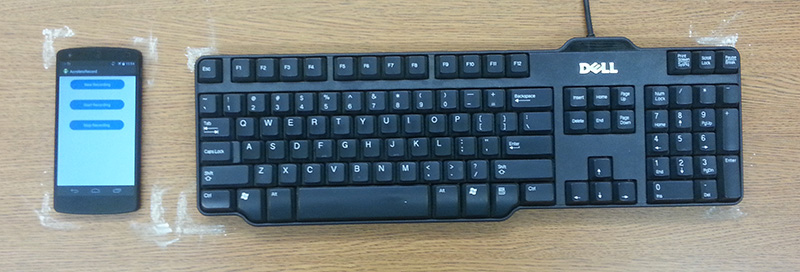
\includegraphics[width=0.5\textwidth]{img/setup}
\caption{Threat model of a smartphone placed next to a keyboard. Used in our experimental setup to capture the dataset.
}
\label{fig:setup}
\end{figure}

\begin{figure}
\centering
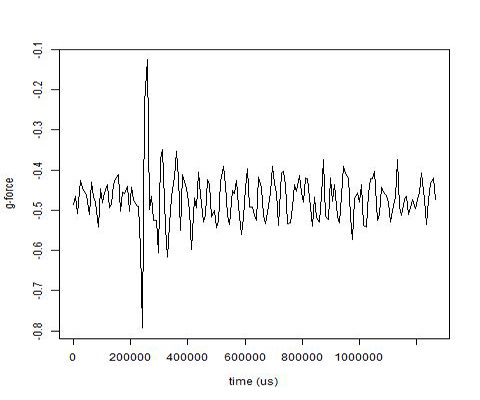
\includegraphics[width=0.5\textwidth]{img/a_162}
\caption{Sample Recording for letter 'a' showing one distinct peak.}
\label{fig:signal-a}
\end{figure}

\begin{figure}
\centering
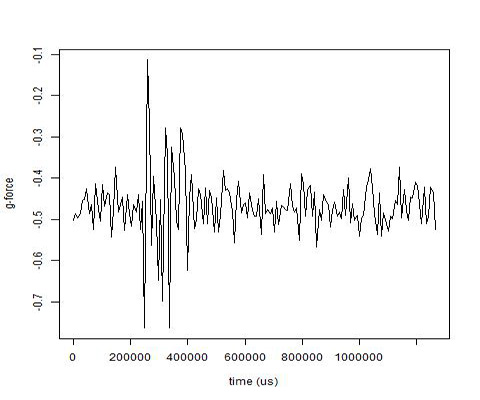
\includegraphics[width=0.5\textwidth]{img/b_147}
\caption{Sample Recording for letter 'b' showing three distinct peaks.}
\label{fig:signal-b}
\end{figure}

\begin{figure}
\centering
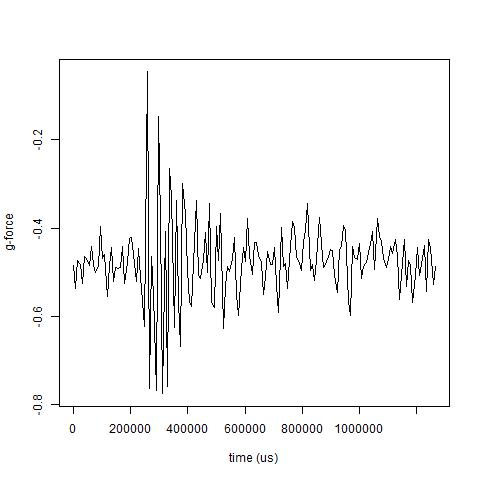
\includegraphics[width=0.5\textwidth]{img/p_566}
\caption{Sample Recording for letter 'p' showing four closely placed peaks.}
\label{fig:signal-p}
\end{figure}

\begin{figure}
\centering
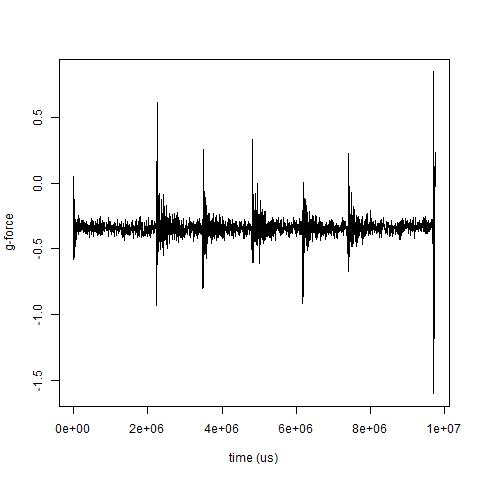
\includegraphics[width=0.5\textwidth]{img/juice}
\caption{Sample Recording for the word ``juice"}
\label{fig:juice}
\end{figure}

\begin{figure*}
\centering
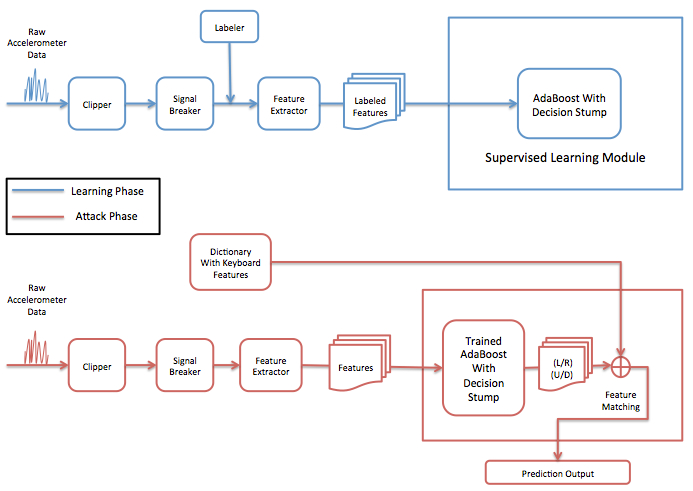
\includegraphics[width=.9\textwidth]{flowchart1}
\caption{The Data Processing Architecture. This diagram provides a high level overview of the architecture used for training the
classifiers and for analyzing keyboard input during an attack.}
\label{fig:flowchart1}
\end{figure*}

\begin{figure*}
\centering
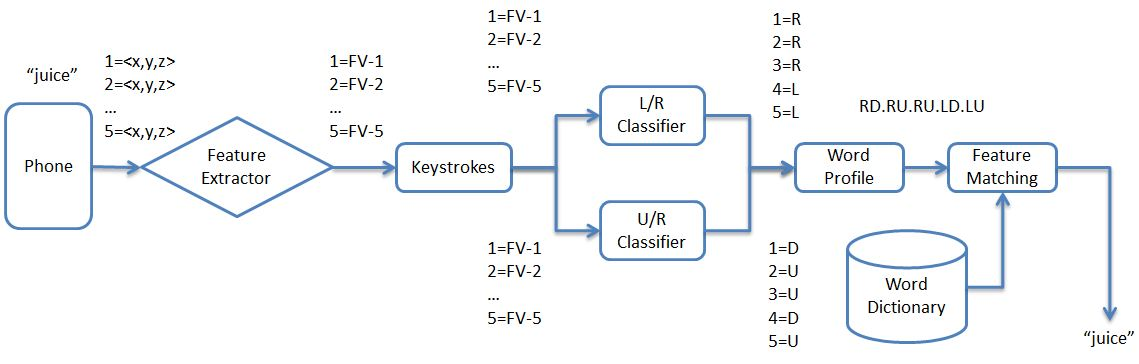
\includegraphics[width=.9\textwidth]{flowchart2}
\caption{Attack Phase Example. Using the word signal from Fig.~\ref{fig:juice}, it runs the clipper to remove noise from
start and end, then extracts the individual letter signals, followed by feature extraction. These are fed to the prediction
model and using the dictionary, the word is found.}
\label{fig:flowchart2}
\end{figure*}

\begin{table}[h]
\centering
{%\small
\resizebox{9cm}{!}{
\begin{tabular}{|c|c|c|}
\hline
\textbf{Dataset} & \textbf{Algorithm} & \textbf{Test Accuracy(\%)}\\
\hline
\multirow{3}{*}{L/R} & AdaBoost (RandomForests) & 68.67\\
\cline{2-3}
& AdaBoost (DecisionStumps) & 69.82\\
\cline{2-3}
& Neural Networks & 68.10\\
\hline
\multirow{3}{*}{U/D} & AdaBoost (RandomForests) & 56.60\\
\cline{2-3}
& AdaBoost (DecisionStumps) & 58.68\\
\cline{2-3}
& Neural Networks & 58.62\\
\hline
\multirow{3}{*}{Triads} & AdaBoost (RandomForests) & 16.37\\
\cline{2-3}
& AdaBoost (DecisionStumps) & 13.21\\
\cline{2-3}
& Neural Networks & 14.65\\
\hline
\end{tabular}
}
}
\caption{Test accuracies of different machine learning algorithms on the test dataset.}
\label{tab:algos-compare}
\end{table}

\begin{table}[h]
\centering
{%\small
\resizebox{9cm}{!}{
\begin{tabular}{|c|c|c|}
\hline
\textbf{Dataset} & \textbf{Features Picked} & \textbf{Test Accuracy(\%)}\\
\hline
\multirow{2}{*}{L/R} & FFTs & 69.54\\
\cline{2-3}
& non-FFTs & 59.48\\
\hline
\multirow{2}{*}{U/D} & FFTs & 56.89\\
\cline{2-3}
& non-FFTs & 59.48\\
\hline
\multirow{2}{*}{Triads} & FFTs & 19.54\\
\cline{2-3}
& non-FFTs & 15.22\\
\hline
\end{tabular}
}
}
\caption{Test accuracies with and without FFT features using AdaBoost with RandomForests.}
\label{tab:ffts-non-ffts}
\end{table}

\begin{table}[h]
\centering
{%\small
\resizebox{9cm}{!}{
\begin{tabular}{|c|c|}
\hline
\textbf{Expected \# of Letter} & \textbf{Percentage of}\\
\textbf{Mis-predictions} & \textbf{Recovered Words(\%)}\\
\hline
0 & 5.46\\
\hline
0.5 & 23.41\\
\hline
1 & 41.64\\
\hline
1.5 & 70.31\\
\hline
2 & 85.67\\
\hline
2.5 & 94.54\\
\hline
3 & 97.27\\
\hline
\end{tabular}
}
}
\caption{Percentage of words recovered with at most the given number of errors in predictions}
\label{tab:harvard-labels}
\end{table}

\begin{figure}
\centering
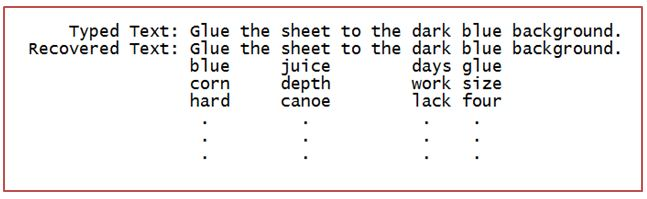
\includegraphics[width=0.5\textwidth]{img/words-options}
\caption{Word options for an Harvard sentence. A word with no options represents the
exactly matching word predictions.}
\label{fig:words-options}
\end{figure}

%ACKNOWLEDGMENTS are optional
%\section*{Acknowledgments}

% An example of a floating figure using the graphicx package.
% Note that \label must occur AFTER (or within) \caption.
% For figures, \caption should occur after the \includegraphics.
% Note that IEEEtran v1.7 and later has special internal code that
% is designed to preserve the operation of \label within \caption
% even when the captionsoff option is in effect. However, because
% of issues like this, it may be the safest practice to put all your
% \label just after \caption rather than within \caption{}.
%
% Reminder: the "draftcls" or "draftclsnofoot", not "draft", class
% option should be used if it is desired that the figures are to be
% displayed while in draft mode.
%
%\begin{figure}[!t]
%\centering
%\includegraphics[width=2.5in]{myfigure}
% where an .eps filename suffix will be assumed under latex, 
% and a .pdf suffix will be assumed for pdflatex; or what has been declared
% via \DeclareGraphicsExtensions.
%\caption{Simulation Results}
%\label{fig_sim}
%\end{figure}

% Note that IEEE typically puts floats only at the top, even when this
% results in a large percentage of a column being occupied by floats.


% An example of a double column floating figure using two subfigures.
% (The subfig.sty package must be loaded for this to work.)
% The subfigure \label commands are set within each subfloat command, the
% \label for the overall figure must come after \caption.
% \hfil must be used as a separator to get equal spacing.
% The subfigure.sty package works much the same way, except \subfigure is
% used instead of \subfloat.
%
%\begin{figure*}[!t]
%\centerline{\subfloat[Case I]\includegraphics[width=2.5in]{subfigcase1}%
%\label{fig_first_case}}
%\hfil
%\subfloat[Case II]{\includegraphics[width=2.5in]{subfigcase2}%
%\label{fig_second_case}}}
%\caption{Simulation results}
%\label{fig_sim}
%\end{figure*}
%
% Note that often IEEE papers with subfigures do not employ subfigure
% captions (using the optional argument to \subfloat), but instead will
% reference/describe all of them (a), (b), etc., within the main caption.


% An example of a floating table. Note that, for IEEE style tables, the 
% \caption command should come BEFORE the table. Table text will default to
% \footnotesize as IEEE normally uses this smaller font for tables.
% The \label must come after \caption as always.
%
%\begin{table}[!t]
%% increase table row spacing, adjust to taste
%\renewcommand{\arraystretch}{1.3}
% if using array.sty, it might be a good idea to tweak the value of
% \extrarowheight as needed to properly center the text within the cells
%\caption{An Example of a Table}
%\label{table_example}
%\centering
%% Some packages, such as MDW tools, offer better commands for making tables
%% than the plain LaTeX2e tabular which is used here.
%\begin{tabular}{|c||c|}
%\hline
%One & Two\\
%\hline
%Three & Four\\
%\hline
%\end{tabular}
%\end{table}


% Note that IEEE does not put floats in the very first column - or typically
% anywhere on the first page for that matter. Also, in-text middle ("here")
% positioning is not used. Most IEEE journals/conferences use top floats
% exclusively. Note that, LaTeX2e, unlike IEEE journals/conferences, places
% footnotes above bottom floats. This can be corrected via the \fnbelowfloat
% command of the stfloats package.


% conference papers do not normally have an appendix


% trigger a \newpage just before the given reference
% number - used to balance the columns on the last page
% adjust value as needed - may need to be readjusted if
% the document is modified later
%\IEEEtriggeratref{8}
% The "triggered" command can be changed if desired:
%\IEEEtriggercmd{\enlargethispage{-5in}}

% references section

% can use a bibliography generated by BibTeX as a .bbl file
% BibTeX documentation can be easily obtained at:
% http://www.ctan.org/tex-archive/biblio/bibtex/contrib/doc/
% The IEEEtran BibTeX style support page is at:
% http://www.michaelshell.org/tex/ieeetran/bibtex/
%\bibliographystyle{IEEEtran}
% argument is your BibTeX string definitions and bibliography database(s)
%\bibliography{IEEEabrv,../bib/paper}
%
% <OR> manually copy in the resultant .bbl file
% set second argument of \begin to the number of references
% (used to reserve space for the reference number labels box)
\clearpage
%\cleardoublepage
\bibliographystyle{unsrt}
\bibliography{sigproc}

%\begin{thebibliography}{1}
%
%\bibitem{IEEEhowto:kopka}
%H.~Kopka and P.~W. Daly, \emph{A Guide to \LaTeX}, 3rd~ed.\hskip 1em plus
%  0.5em minus 0.4em\relax Harlow, England: Addison-Wesley, 1999.
%
%\end{thebibliography}
%\appendix
%Appendix A

%\section{Appendix Section}

%\subsection{Appendix Subsection}

%\balancecolumns




% that's all folks
\end{document}


